% !TEX TS-program = xelatex

\documentclass{beamer}
\usetheme{default}

\usepackage{ctex}

\title{FMA: A DATASET FOR MUSIC ANALYSIS\\(ISMIR 2017)}
\author{张展鹏}
\begin{document}
\begin{frame}[plain]
    \maketitle
\end{frame}

\begin{frame}{为什么音乐分析数据库是必要的?}
	\textbf{MIR == Music Information Retrieval}
	\begin{itemize}
		\item 特征和端到端学习需要大型音乐数据集。
		\item 大型音乐数据集需要实现浏览、搜索和组织等功能。
		\item Free,源代码和数据集均开放;Archive,数据集规模很大。
	\end{itemize}
\end{frame}

\begin{frame}{FMA的特点}
	\textbf{FMA == Free Music Archive}
	\begin{itemize}
		\item Free,源代码和数据集均开放;Archive,数据集规模很大。
		\item FMA提供了917GB的数据集和343天的知识共享许可。
		\item 这些音频来自16341位艺术家的106574首曲目和14854张专辑,按 161种流派分层分类。
		\item FMA提供了完整长度和高质量的音频及特征,以及级元数据、标签和简介文本等数据。
	\end{itemize}
\end{frame}

\begin{frame}{论文工作简述}
	\begin{itemize}
		\item 对比现有工作,实现FMA相关系统设计。
		\item 为MIR任务提供训练、验证和测试集并评估效果。
		\item 对音乐进行流派识别。
	\end{itemize}
\end{frame}

\begin{frame}{FMA跟同类音乐数据库比较}
	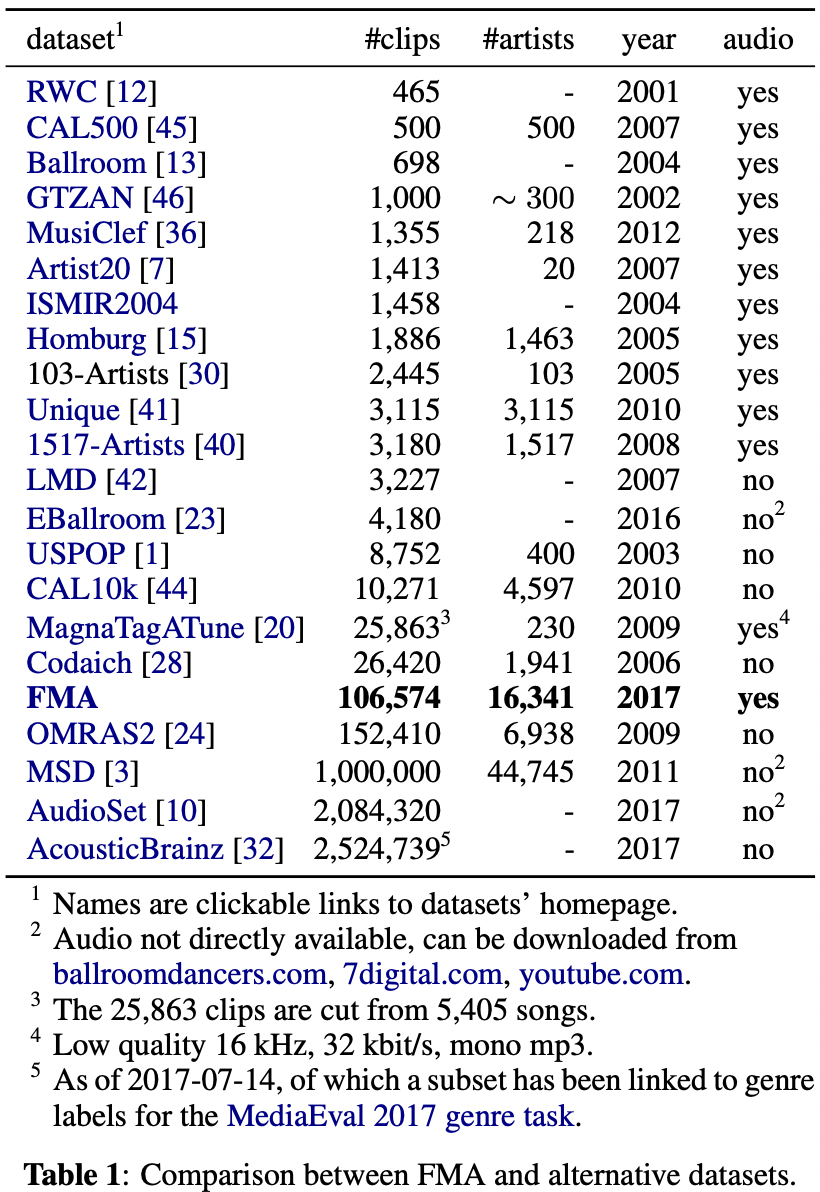
\includegraphics[width=0.5\linewidth]{Assets/表1}
\end{frame}

\begin{frame}{音乐分析数据库的需求(1)——数据规模大}
	音乐分析数据库需要大规模数据集来避免过拟合。
	\begin{itemize}
		\item 一般地,样本容量越大,拟合结果越好。
		\item 大规模数据更接近真实,数据更平衡。数据的缺点包含噪声以及其他可能被模型利用的、跟基本事实混淆的特征。
	\end{itemize}
	FMA的数据规模足够大。
\end{frame}

\begin{frame}{音乐分析数据库的需求(2)——版权}
	一般地,唱片公司会对音乐加以严格的版权限制。
	\begin{itemize}
		\item CC == Creative Commons (license),知识共享许可协议。
		\item BY == Attribution,署名;您(用户)可以复制、发行、展览、表演、放映、广播或通过信息网络传播本作品;您必须按照作者或者许可人指定的方式对作品进行署名。
		\item 4.0,发布日期是2013年11月25日;它不需要移植就可以适用于各地的法律,4.0版并不鼓励移植,而是希望能作为一个全球通用的许可方式。
		\item MIT,作者是麻省理工学院;与其他常见的软件许可协议(如GPL、LGPL、BSD)相比,它是相对宽松的软件许可协议。
	\end{itemize}
	FMA收集版权许可的音轨并重新分发。数据在CC BY 4.0下获得许可;源代码在MIT下获得许可。
\end{frame}

\begin{frame}{音乐分析数据库的需求(3)——音频可下载}
	我们希望音乐分析数据库足够大,同时有原始音频可供自由分析。
	\begin{itemize}
		\item 较小的数据集通常会分发音频,大多数较大的数据集不会。
		\item 某些数据集仅分发部分从音频提取的特征,它们的用途受到了限制。
		\item 某些数据集仅提供下载链接,这样的下载资源不受控制,可能被移除。
	\end{itemize}
	FMA较新,直接提供了音频。
\end{frame}

\begin{frame}{音乐分析数据库的需求(4)——音频质量好}
	音频质量有剪辑时长和采样率这2个主要指标。
	\begin{itemize}
		\item 其他音乐分析数据库通常提供10-30s的剪辑,这会导致同一首曲目的不同剪辑可能导致不一样的预测结果;另外,研究人员难以自由截取音频片段。
		\item 某些音乐分析数据库的比特率低至32kbit/s;主流数据库,例如MSD,比特率为104kbit/s。
	\end{itemize}
	FMA的文件名称是音轨ID,以mp3格式编码。大多数采样率为44100Hz,比特率为 320kbit/s(平均为263kbit/s),并且是立体声的。
\end{frame}

\begin{frame}{音乐分析数据库的需求(5)——元数据丰富}
	FMA在元数据覆盖率上具有显著优势。
	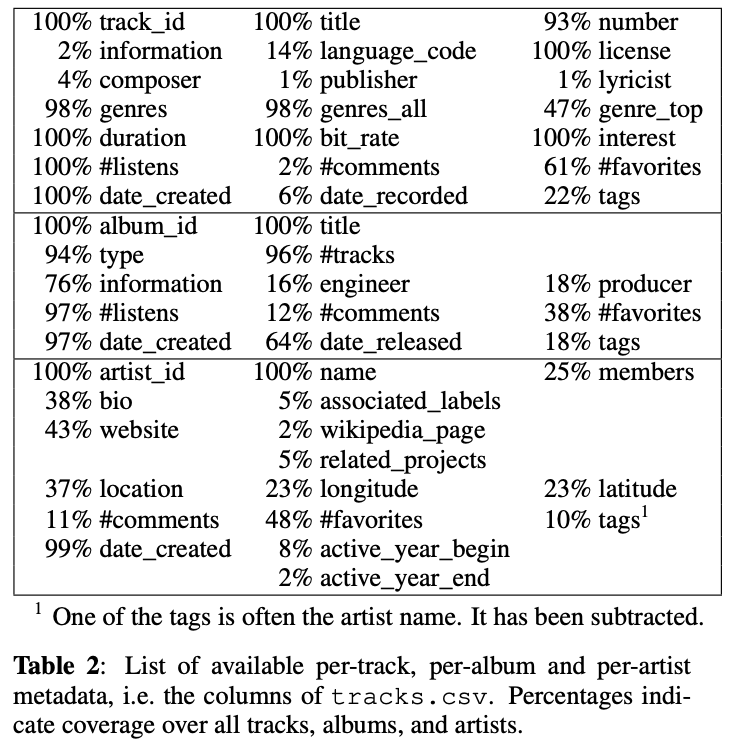
\includegraphics[width=0.6\linewidth]{Assets/表2}
\end{frame}

\begin{frame}{音乐分析数据库的需求(6)——容易获取}
	FMA易于访问。它的数据集只包含CSV格式记录的元数据和和MP3格式的音频,可以直接下载。
\end{frame}

\begin{frame}{音乐分析数据库的需求(7)——数据存档、易配置}
	FMA的全体文件和档案都经过校验并存档托管;公开了用于
	\begin{itemize}
		\item (i)收集数据,
		\item (ii)分析数据,
		\item (iii)生成子集和拆分,
		\item (iv)计算特征,
		\item (v)测试基线
	\end{itemize}
	的所有源代码。这些源代码容易被修改以被研究人员用于计算自己的特征和评估自己的方法。另外,依赖于公共曲库和API,任何人都可以重新创建或扩展曲库。
\end{frame}

\begin{frame}{FMA的规模}
	\begin{itemize}
		\item 截止2017年4月1日,最大音轨ID高达155320,其中109727首是有效的,丢失的45594首可能对应已删除的曲目。
		\item 在109727首有效的音轨中,180首无法下载,286首无法被 ffmpeg剪辑,71首无法用以提取特征,2616首的许可证禁止重新分发,剩下106574首可以自由使用。
		\item FMA未人为筛选音轨,以去除流派过多、过长、和稀有流派等曲目。这样做是为了使音轨分布接近真实情况。
	\end{itemize}
\end{frame}

\begin{frame}{FMA的成长}
	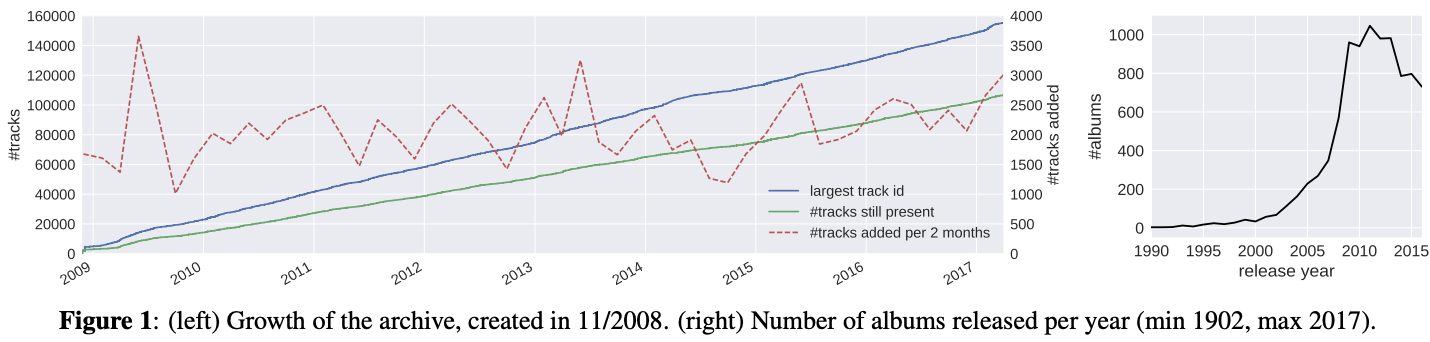
\includegraphics[width=\linewidth]{Assets/图1}
\end{frame}

\begin{frame}{依赖元数据构建关系型数据库}
	元数据被清理和格式化,构建关系型数据库。
	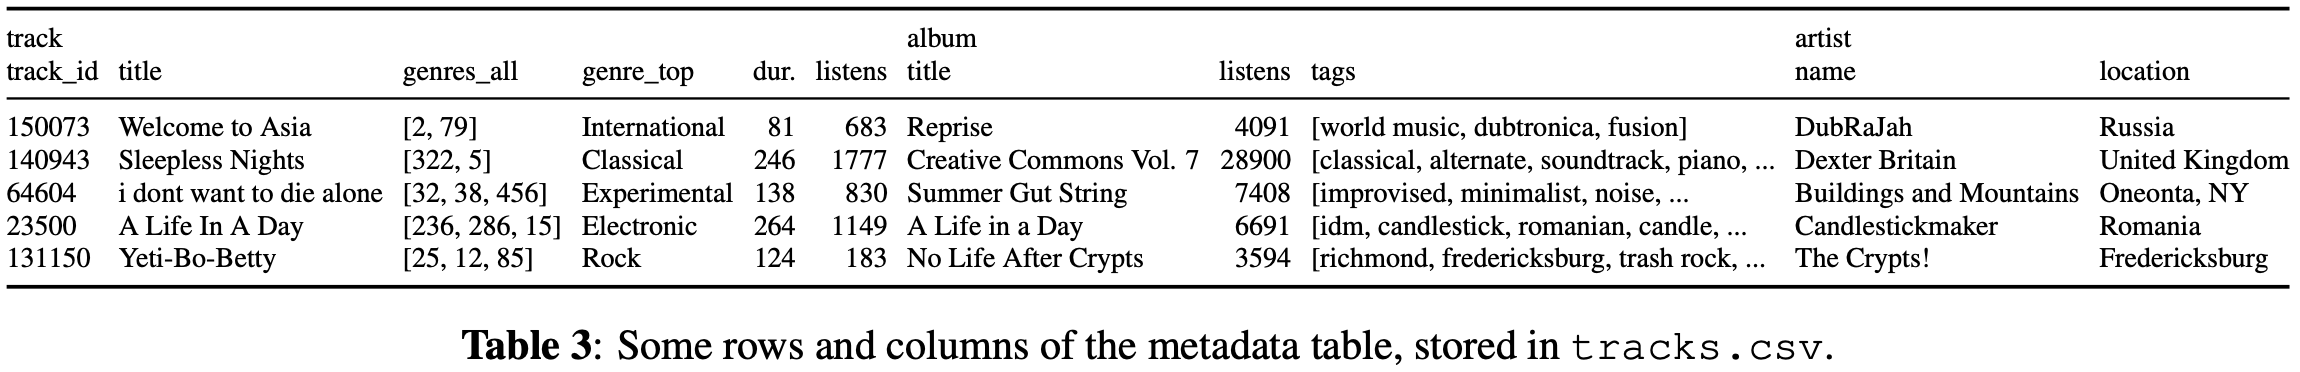
\includegraphics[width=\linewidth]{Assets/表3}
\end{frame}

\begin{frame}{音轨时长和播放量分布}
	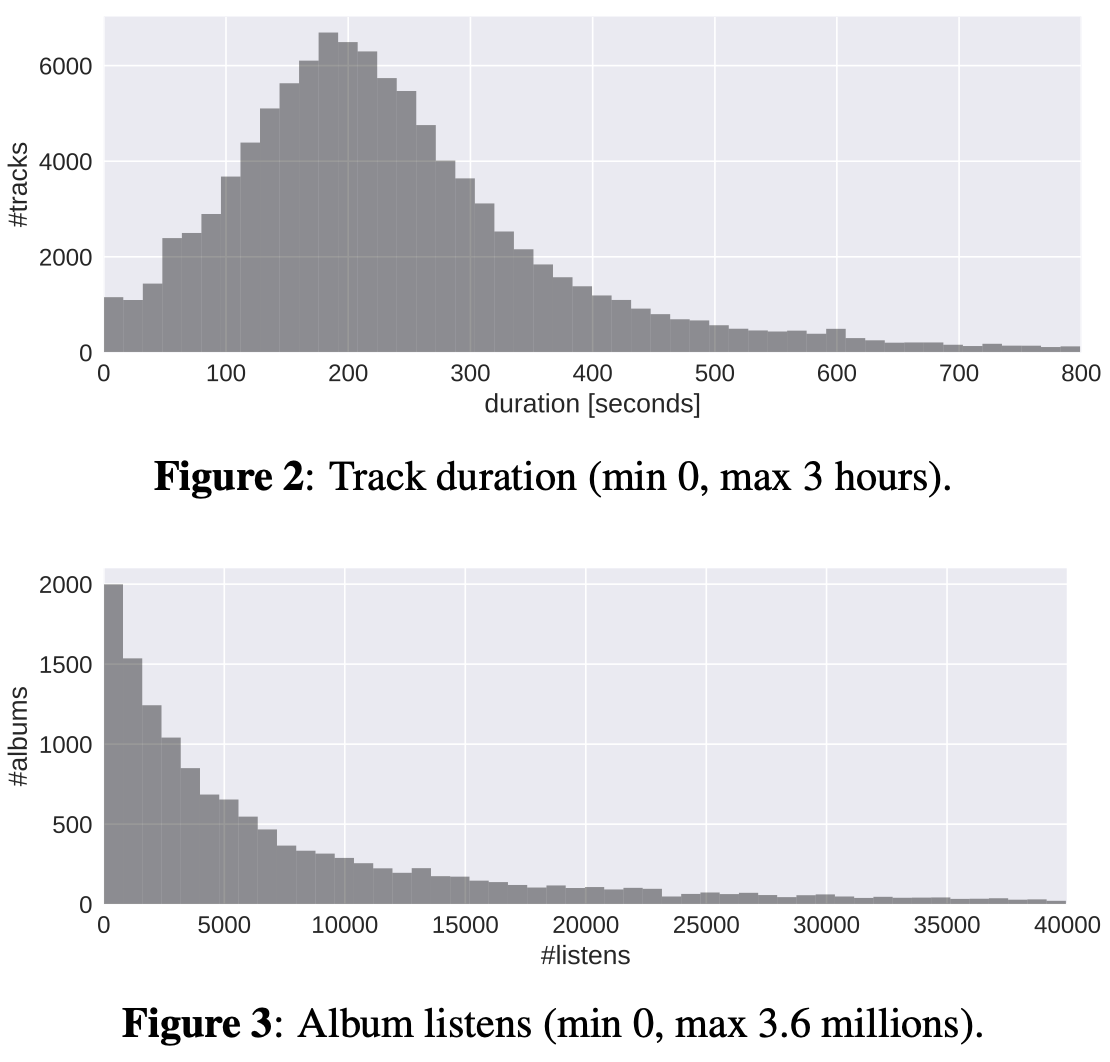
\includegraphics[width=0.8\linewidth]{Assets/图2_3}
\end{frame}

\begin{frame}{流派分类}
	FMA具有精细的流派信息——内置的层次结构,并且由艺术家自行注释;也可以由众包和专家来补充。
	\begin{itemize}
		\item 标签噪声是不可避免的。
		\item 流派标签的层次结构由161个流派组成,其中16个是根流派,其他是子流派。
	\end{itemize}
\end{frame}

\begin{frame}{流派分层分类举例(1)}
	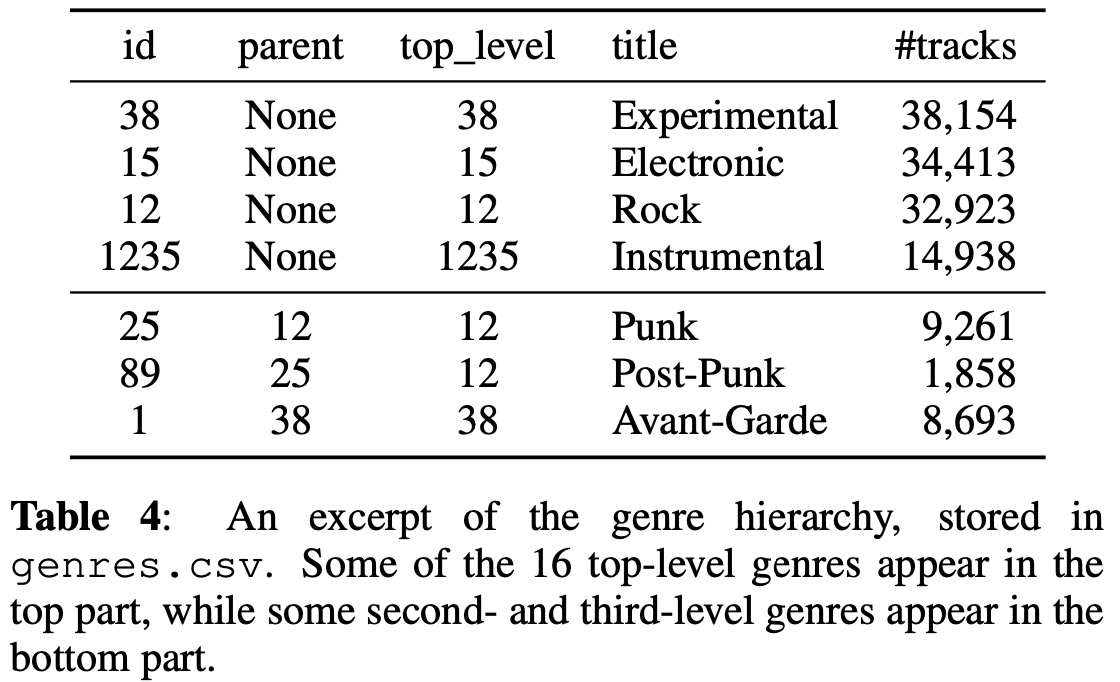
\includegraphics[width=\linewidth]{Assets/表4}
\end{frame}

\begin{frame}{流派分层分类举例(2)}
	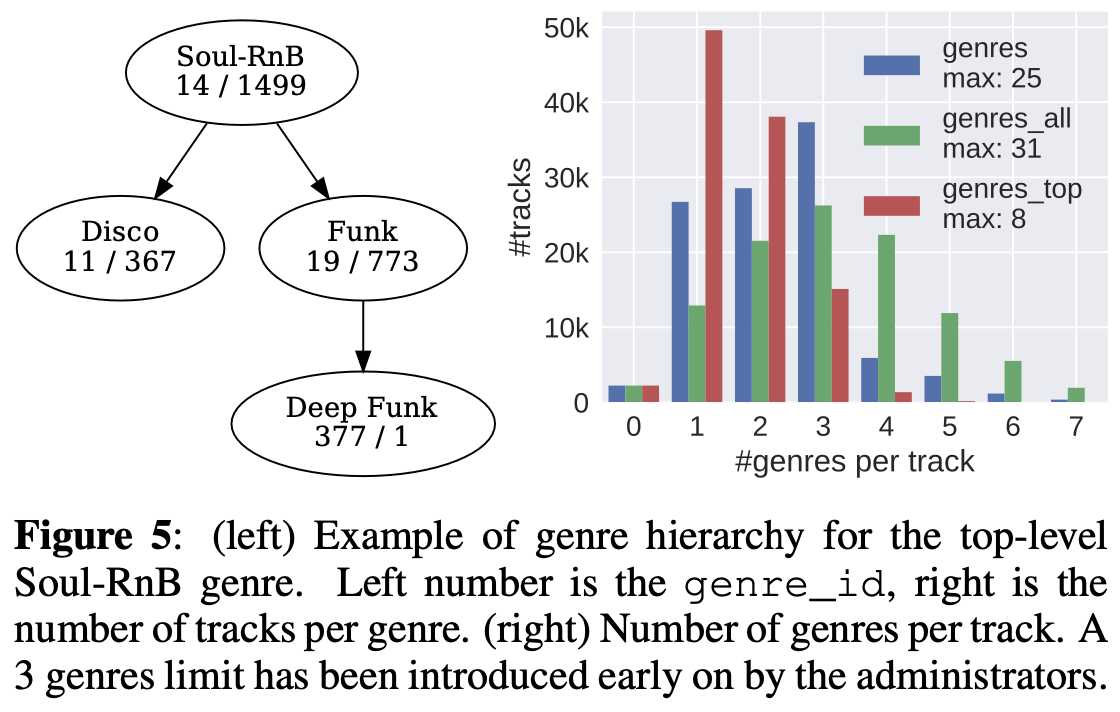
\includegraphics[width=\linewidth]{Assets/图5}
\end{frame}

\begin{frame}{特征提取——流派分类统计}
	流派分类任务是预先进行的。\\
	Each feature set (except zero-crossing rate) is computed on windows of 2048 samples spaced by hops of 512 samples. Seven statistics were then computed over all windows: the mean, standard deviation, skew, kurtosis, median, minimum and maximum.\\
	平均值、标准偏差、偏斜、峰度、中值、最小值和最大值
	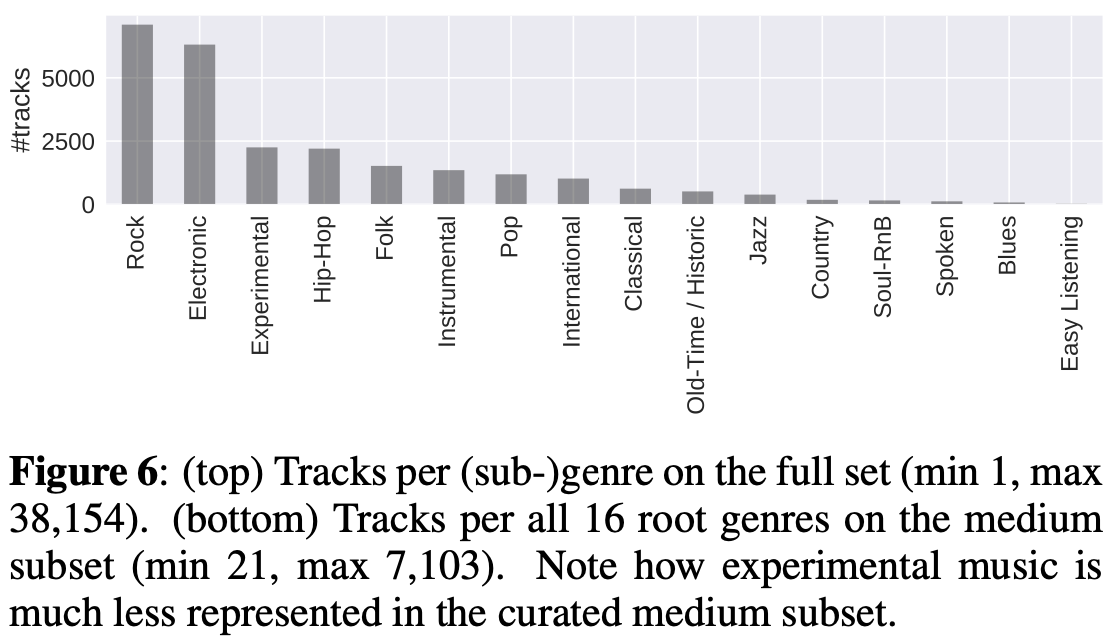
\includegraphics[width=0.8\linewidth]{Assets/图6}
\end{frame}

\begin{frame}{子数据集——Small, medium, large and full}
	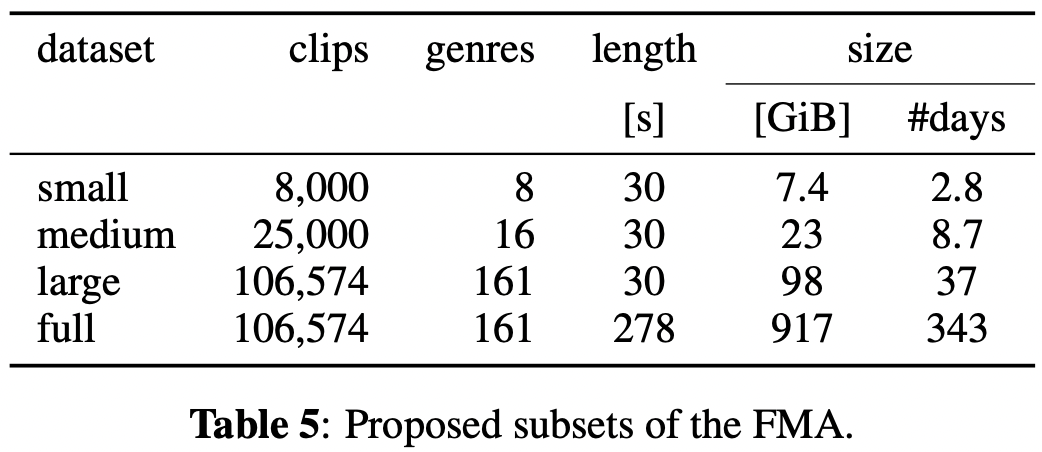
\includegraphics[width=\linewidth]{Assets/表5}
\end{frame}

\begin{frame}{数据集划分与抽样方法}
	经典分割:训练集:验证集:测试集 = 8:1:1。
	为了使使用FMA的结果可重现,如果使用交叉验证,则应合并训练集和验证集。数据集划分应该满足下列约束条件:
	\begin{itemize}
		\item 每个根流派均保证在所有分组(split)中表示。
		\item 较小的流派子集会满足8:1:1的划分比例;但不保证最小的7个子流派出现在所有分组中。
		\item 因为同一个艺术家的歌曲同时出现在训练和测试集会导致分类准确性比实际表现得乐观,所以同一个艺术家的歌曲只会出现在单个分组中。
		\item 没有流派标签的2231首歌曲会被完全分配给训练集用于搬家度学习,以及作为额外的训练样本。
	\end{itemize}
\end{frame}

\begin{frame}{FMA的用途举例}
	\begin{itemize}
		\item 音乐分类和注释。包括流派识别、艺术家识别、年份预测和特点自动标记等。
		\item 流派识别。音乐流派是通过文化、艺术家和市场力量的复杂相互作用而产生的类别,用于表征作品之间的相似性。
		\item 数据分析。这一步主要指分析音频。FMA的完整曲目可用性允许对音乐属性进行适当的研究,例如音乐结构分析;元数据是对现有数据集的有价值补充,用以元数据分析。
	\end{itemize}
\end{frame}

\begin{frame}{FMA设计与实现的结论}
	\begin{itemize}
		\item FMA是一个可以在研究人员之间轻松共享的数据集。
		\item FMA允许用户对数据进行自由的定义和拆分。
		\item FMA的样本容量足够大,这意味着FMA提供的样本几乎不会出现不平衡的问题,足够接近真实情况。
		\item FMA适合用以音乐流派识别,即MGR。
		\item 曲库也是知识库,共享是第一位的,这会方便教育和研究。
	\end{itemize}
\end{frame}

\begin{frame}
	谢谢!
\end{frame}
\end{document}
